\documentclass[tikz,border=0pt]{standalone}
\usepackage[utf8]{inputenc}
\usepackage[T1]{fontenc}
\usepackage{lmodern}
\usepackage{xcolor}
\definecolor{BMEgreen}{RGB}{85, 157, 0}
\definecolor{BMEred}{RGB}{209, 0, 0}
\definecolor{TechCyan}{RGB}{0, 110, 180}

\begin{document}
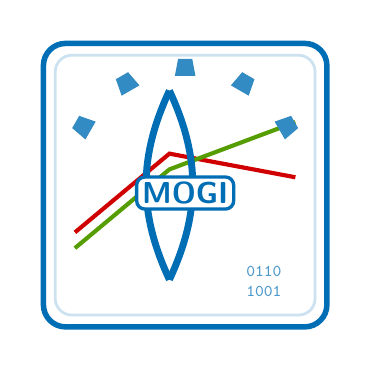
\begin{tikzpicture}
  \path[use as bounding box] (0, 0) rectangle (4, 4);
  \fill[white] (0, 0) rectangle (4, 4);

  \begin{scope}[shift={(2, 2)}]
    % Outer rounded technical frame
    \draw[TechCyan, line width=2pt, rounded corners=8pt] (-1.8, -1.8) rectangle (1.8, 1.8);
    \draw[TechCyan!20, line width=1pt, rounded corners=6pt] (-1.65, -1.65) rectangle (1.65, 1.65);

    % Optical rays / lens beam (Optics)
    \draw[BMEred, line width=1.5pt] (-1.4, -0.6) -- (-0.2, 0.4) -- (1.4, 0.1);
    \draw[BMEgreen, line width=1.5pt] (-1.4, -0.8) -- (-0.2, 0.2) -- (1.4, 0.8);
    
    % Lens element (vertical curve)
    \draw[TechCyan, line width=2.5pt] (-0.2, -1.2) to[bend left=25] (-0.2, 1.2);
    \draw[TechCyan, line width=2.5pt] (-0.2, -1.2) to[bend right=25] (-0.2, 1.2);

    % Mechatronics / Gear sector
    \foreach \a in {30, 60, ..., 150} {
      \draw[fill=TechCyan!80, draw=TechCyan!80] (\a-5:1.4) -- (\a-3:1.6) -- (\a+3:1.6) -- (\a+5:1.4) -- cycle;
    }

    % Informatics bit pattern (0 1 0 1)
    \node[TechCyan!70, font=\fontsize{6}{7}\ttfamily\bfseries] at (1.0, -1.1) {0110};
    \node[TechCyan!70, font=\fontsize{6}{7}\ttfamily\bfseries] at (1.0, -1.35) {1001};

    % MOGI text badge
    \node[fill=white, draw=TechCyan, line width=1.2pt, rounded corners=3pt, inner sep=2pt] at (0, -0.1) {%
      \textcolor{TechCyan}{\fontsize{11}{13}\sffamily\bfseries MOGI}%
    };
  \end{scope}
\end{tikzpicture}
\end{document}
